\section{Territorial analysis I (Exercise 1.2)}\label{sec:territorial-I}
\noindent Responsible: Person A. Notebook: \code{notebooks/ex12\_territorial\_analysis\_I.ipynb}.

\paragraph{Data sources.}
Two census products are combined, and every number below states which one it comes from.
\begin{itemize}
  \item The \emph{detailed census} RP2019~\cite{insee-census-detailed} (171{,}834 observations for Calvados, weights
  \code{IPONDI}) has single-year ages and the SPC of every person, but identifies only 17 of the 528 municipalities
  (\cref{sec:study-area}). It is used for all department-level statistics, with weights.
  \item The \emph{aggregated census by IRIS} RP2019 ``Population en 2019 -- IRIS''~\cite{insee-census-aggregated}
  (656 IRIS in Calvados, aggregated to municipalities with the code
  \code{COM}) covers all 528 municipalities, with ten age bands and the population aged 15 and over by SPC. Its counts
  are already weighted by INSEE. It is used for every statistic of a single municipality. Its 528 municipality codes
  are identical to those of IGN CONTOURS-IRIS 2021 (no mismatch on either side).
\end{itemize}
The age bands of the aggregated file add up to its population \code{P19\_POP} in every municipality, and the eight SPC
counts add up to the population 15+ \code{C19\_POP15P}. \code{P19\_POP} sums to 694{,}905 persons, exactly the official
population municipale~\cite{insee-popleg-2019}, 227 persons (0.03\,\%) less than the weighted total of the detailed
file. The SPC counts (\code{C19\_*}) come from the same sample of answers (\emph{exploitation compl\'ementaire}) as the
detailed file: its weighted population aged 15+ (576{,}234) is identical to \code{C19\_POP15P}.

\paragraph{Age variable.}
The detailed file has two single-year ages: \code{AGED}, the census year minus the year of birth (\emph{\^age en
diff\'erence de mill\'esimes}), and \code{AGEREV}, the age in completed years (\emph{\^age en ann\'ees r\'evolues}).
We use \code{AGEREV} throughout. It is the usual meaning of age, and it is the variable behind the age bands of the
aggregated file: with \code{AGEREV} the weighted band totals of the detailed file agree with the aggregated totals
within 1.0\,\% in every band, with \code{AGED} they differ by up to 33\,\% (band 0--2 years).

\subsection{Age distribution and average age (1 point)}

\paragraph{Method.}
For each age $a$ (completed years) the number of persons is the sum of the weights of the observations of that age,
$N_a = \sum_{k:\,a_k = a} w_k$, over all 171{,}834 observations of the department. The average age is the weighted mean
$\bar a = \sum_k w_k a_k / \sum_k w_k$; we also report the weighted median.

\begin{figure}[H]
  \centering
  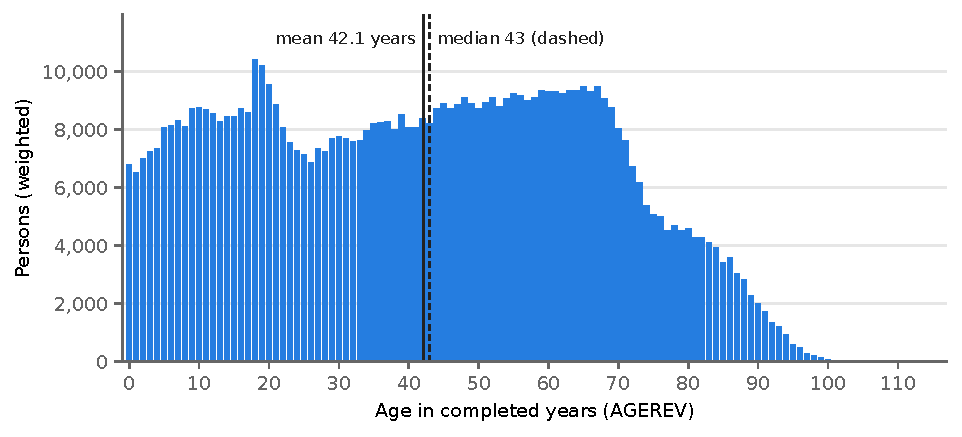
\includegraphics[width=\textwidth]{age_distribution}
  \caption{Weighted age distribution of the population of Calvados (persons per single year of age, \code{AGEREV}),
  with the weighted mean (solid) and median (dashed). Data: INSEE RP2019 detailed census~\cite{insee-census-detailed},
  weights \code{IPONDI}.}
  \label{fig:age-distribution}
\end{figure}

\paragraph{Result.}
The \textbf{average age of the persons living in Calvados is 42.1 years} (weighted mean of \code{AGEREV}); the median is
43 years. With \code{AGED} the mean would be 43.0 years, about one year more, because \code{AGED} counts the birthday of
the census year in advance. \Cref{fig:age-distribution} shows a sharp peak at 18--19 years, a trough in the mid-twenties
(minimum at 26 years), and a broad plateau from about 45 to 68 years (the baby-boom cohorts), followed by a steep
decline after 70. The peak at 18--19 reflects young people who come to study in Caen; the trough means that many of
them leave again after their studies. 21.5\,\% of the population is 65 or older and 23.8\,\% is younger than 20.
Without weights the mean age would be 41.2 years, 0.8 years too low: observations in the large municipalities, which
are younger (\cref{tab:mean-age-validation}), carry smaller weights (\cref{tab:study-area-weights}) and are therefore
over-represented among the rows.

\subsection{Average age per municipality, youngest and oldest (1 point)}

\paragraph{Method.}
Because the detailed file identifies only 17 municipalities (37.7\,\% of the population, \cref{sec:study-area}), a
map of all 528 municipalities cannot be built from it. The average age per municipality is therefore estimated from
the ten age bands of the aggregated census (0--2, 3--5, 6--10, 11--17, 18--24, 25--39, 40--54, 55--64, 65--79 and
80 years or more). Every person of a band $b$ is given the band midpoint $m_b = (l_b + u_b)/2$ in completed years
(e.g.\ 32 for 25--39). For the open band 80+ we assume $m_b = 85$ years; in the detailed file the actual weighted mean
age of this band is 85.7 years. The estimate for municipality $i$ is
$\hat a_i = \sum_b m_b P_{ib} / \sum_b P_{ib}$, where $P_{ib}$ is the population of $i$ in band $b$ and
$\sum_b P_{ib}$ equals \code{P19\_POP}.

\paragraph{Validation.}
For the department and the 17 identifiable municipalities we compare the exact weighted mean age from single-year
ages with the band estimate applied to the same persons of the detailed file (\cref{tab:mean-age-validation}). The
difference is the error of the band approximation alone: 0.08 years for the department, between $-0.16$ and $+0.28$
years for the municipalities (mean $+0.08$). The band estimate from the aggregated file is also shown. It adds the
difference between the two exploitations of the census and deviates by up to 1.1 years (Colombelles), but it ranks
the 17 municipalities almost identically (Spearman correlation 0.99). The approximation is therefore accurate enough
to compare municipalities.

\begin{table}[H]
  \centering
  \caption{Mean age (years): exact weighted mean from single-year ages vs.\ band-midpoint estimate, for the department
  and the 17 municipalities identifiable in the detailed census, sorted by exact mean age. Error = estimate $-$ exact.}
  \label{tab:mean-age-validation}
  \small
  \begin{tabular}{@{}lrrrrr@{}}
    \toprule
    & \multicolumn{3}{c}{Detailed census} & \multicolumn{2}{c}{Aggregated census} \\
    \cmidrule(lr){2-4}\cmidrule(l){5-6}
    Area & Exact & Bands & Error & Bands & Error \\
    \midrule
    \textbf{Calvados (department)} & \textbf{42.05} & \textbf{42.13} & \textbf{+0.08} & \textbf{42.06} & \textbf{+0.01} \\
    \midrule
    H\'erouville-Saint-Clair & 37.85 & 38.13 & +0.28 & 38.11 & +0.26 \\
    Caen & 38.72 & 38.98 & +0.25 & 38.99 & +0.27 \\
    Ifs & 39.23 & 39.40 & +0.18 & 39.38 & +0.15 \\
    Fleury-sur-Orne & 40.66 & 40.79 & +0.13 & 40.96 & +0.30 \\
    Colombelles & 41.18 & 41.41 & +0.23 & 40.09 & $-$1.09 \\
    Giberville & 41.65 & 41.59 & $-$0.06 & 41.49 & $-$0.15 \\
    Mondeville & 42.64 & 42.89 & +0.25 & 42.51 & $-$0.13 \\
    Honfleur & 43.15 & 43.21 & +0.06 & 43.47 & +0.32 \\
    Falaise & 43.46 & 43.32 & $-$0.14 & 43.75 & +0.29 \\
    Lisieux & 43.49 & 43.50 & +0.01 & 43.51 & +0.03 \\
    Cormelles-le-Royal & 44.81 & 45.00 & +0.20 & 44.20 & $-$0.61 \\
    Dives-sur-Mer & 45.66 & 45.66 & +0.00 & 46.12 & +0.46 \\
    Cond\'e-en-Normandie & 45.76 & 45.83 & +0.07 & 45.87 & +0.11 \\
    Vire Normandie & 46.53 & 46.59 & +0.06 & 46.55 & +0.02 \\
    Bayeux & 47.09 & 47.18 & +0.09 & 47.16 & +0.07 \\
    Ouistreham & 50.67 & 50.51 & $-$0.16 & 49.97 & $-$0.69 \\
    Trouville-sur-Mer & 52.39 & 52.27 & $-$0.12 & 52.02 & $-$0.37 \\
    \bottomrule
  \end{tabular}
\end{table}

\begin{figure}[H]
  \centering
  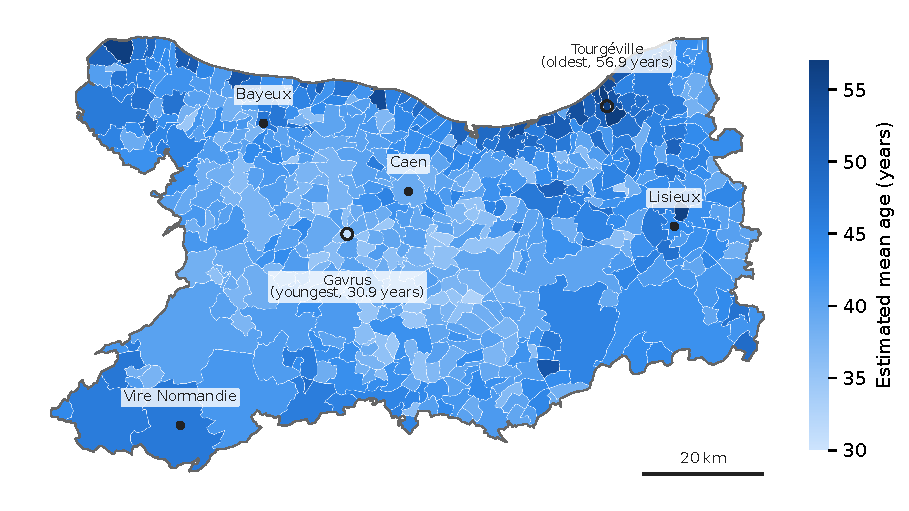
\includegraphics[width=\textwidth]{mean_age_map}
  \caption{Estimated mean age (years) of the population of the 528 municipalities of Calvados, from the age bands of
  the aggregated census RP2019 (band midpoints, 80+ set to 85 years). Circles: youngest and oldest municipality with at
  least 500 inhabitants. Data: INSEE~\cite{insee-census-aggregated}, IGN CONTOURS-IRIS 2021~\cite{ign-contours-iris};
  Lambert-93.}
  \label{fig:mean-age-map}
\end{figure}

\paragraph{Result.}
The estimated mean age of the municipalities ranges from 30.9 to 56.9 years (median 41.4). We name the youngest and the
oldest municipality (a)~over all 528 municipalities and (b)~over the 242 municipalities with at least 500 inhabitants
(90.2\,\% of the population), because the mean age of a municipality of a few dozen inhabitants depends on a handful
of households (\cref{tab:youngest-oldest}). Both variants give the same answer:
\begin{itemize}
  \item \textbf{Youngest: Gavrus} (14297), 584 inhabitants, estimated mean age 30.9 years;
  \item \textbf{Oldest: Tourg\'eville} (14701), 782 inhabitants, estimated mean age 56.9 years.
\end{itemize}
The threshold changes the rest of the ranking: without it, very small municipalities such as Soignolles (128
inhabitants) and Le Fournet (71) appear among the youngest, and Rocques (289) among the oldest.

\begin{table}[H]
  \centering
  \caption{The five youngest and five oldest municipalities by estimated mean age (aggregated census RP2019),
  (a)~all municipalities and (b)~municipalities with at least 500 inhabitants. Population: \code{P19\_POP}.}
  \label{tab:youngest-oldest}
  \small
  \begin{tabular}{@{}llrr@{\hspace{2em}}llrr@{}}
    \toprule
    \multicolumn{4}{c}{(a) All 528 municipalities} & \multicolumn{4}{c}{(b) $\geq$ 500 inhabitants (242)} \\
    \cmidrule(r{2em}){1-4}\cmidrule{5-8}
    Code & Municipality & Pop. & Age & Code & Municipality & Pop. & Age \\
    \midrule
    \multicolumn{8}{@{}l}{\emph{Youngest}} \\
    14297 & Gavrus & 584 & 30.9 & 14297 & Gavrus & 584 & 30.9 \\
    14674 & Soignolles & 128 & 32.8 & 14092 & Bourgu\'ebus & 2{,}186 & 34.2 \\
    14285 & Le Fournet & 71 & 33.6 & 14396 & Maltot & 1{,}024 & 34.6 \\
    14092 & Bourgu\'ebus & 2{,}186 & 34.2 & 14039 & Barbery & 824 & 34.9 \\
    14082 & La Boissi\`ere & 189 & 34.5 & 14207 & Croisilles & 646 & 35.1 \\
    \midrule
    \multicolumn{8}{@{}l}{\emph{Oldest}} \\
    14220 & Deauville & 3{,}565 & 54.6 & 14754 & Villers-sur-Mer & 2{,}543 & 53.9 \\
    14191 & Courseulles-sur-Mer & 4{,}196 & 54.8 & 14220 & Deauville & 3{,}565 & 54.6 \\
    14540 & Rocques & 289 & 56.3 & 14191 & Courseulles-sur-Mer & 4{,}196 & 54.8 \\
    14312 & Grandcamp-Maisy & 1{,}536 & 56.8 & 14312 & Grandcamp-Maisy & 1{,}536 & 56.8 \\
    14701 & Tourg\'eville & 782 & 56.9 & 14701 & Tourg\'eville & 782 & 56.9 \\
    \bottomrule
  \end{tabular}
\end{table}

\Cref{fig:mean-age-map} shows a clear spatial pattern. The oldest municipalities lie on the coast: the seaside resorts
of the C\^ote Fleurie (Tourg\'eville, Deauville, Villers-sur-Mer, Trouville-sur-Mer) and of the C\^ote de Nacre and the
Bessin (Courseulles-sur-Mer, Grandcamp-Maisy), which attract retirees. The youngest are the peri-urban municipalities
around Caen (Gavrus, Maltot, Bourgu\'ebus, Barbery and Croisilles, the light ring south of the city on the map), where
families with children settle. Caen itself and H\'erouville-Saint-Clair are also young (mean ages of 39.0 and 38.1
years in the aggregated file), because of their students and young working population.

\subsection{Socio-professional categories: study area and at least three municipalities (1 point)}

\paragraph{Method.}
All shares refer to the \textbf{population aged 15 and over}, so that the department and the municipalities are
comparable. The SPC counts of the aggregated census are only given for persons aged 15+, and in the detailed file
persons under 15 carry \code{CS1 = 8} (``autres personnes sans activit\'e professionnelle''); without the filter all
children would be counted in category~8. For the \emph{department} we compute the weighted shares of the eight SPCs
from the detailed file (\code{AGEREV} $\geq 15$, weights \code{IPONDI}); the same shares from the aggregated file agree
to within $10^{-14}$ percentage points, as expected since both come from the same exploitation. For the
\emph{municipalities} we use the aggregated file, so that all four areas come from the same source. We chose four
municipalities with contrasting profiles:
\begin{itemize}
  \item \textbf{Caen} (14118, 106{,}230 inhabitants): the main city, regional capital and university town;
  \item \textbf{H\'erouville-Saint-Clair} (14327, 22{,}555): the largest suburb of Caen;
  \item \textbf{Trouville-sur-Mer} (14715, 4{,}603): a seaside resort on the C\^ote Fleurie;
  \item \textbf{\'Epaney} (14240, 511): a rural municipality, chosen by a rule: among the 138 municipalities with
  500 to 1{,}500 inhabitants, the one with the highest share of farmers.
\end{itemize}
The first three are also identifiable in the detailed file, and their weighted shares there are identical to the
aggregated ones. \Cref{fig:spc-distribution} and \cref{tab:spc-shares} compare the shares with the department.

\begin{figure}[H]
  \centering
  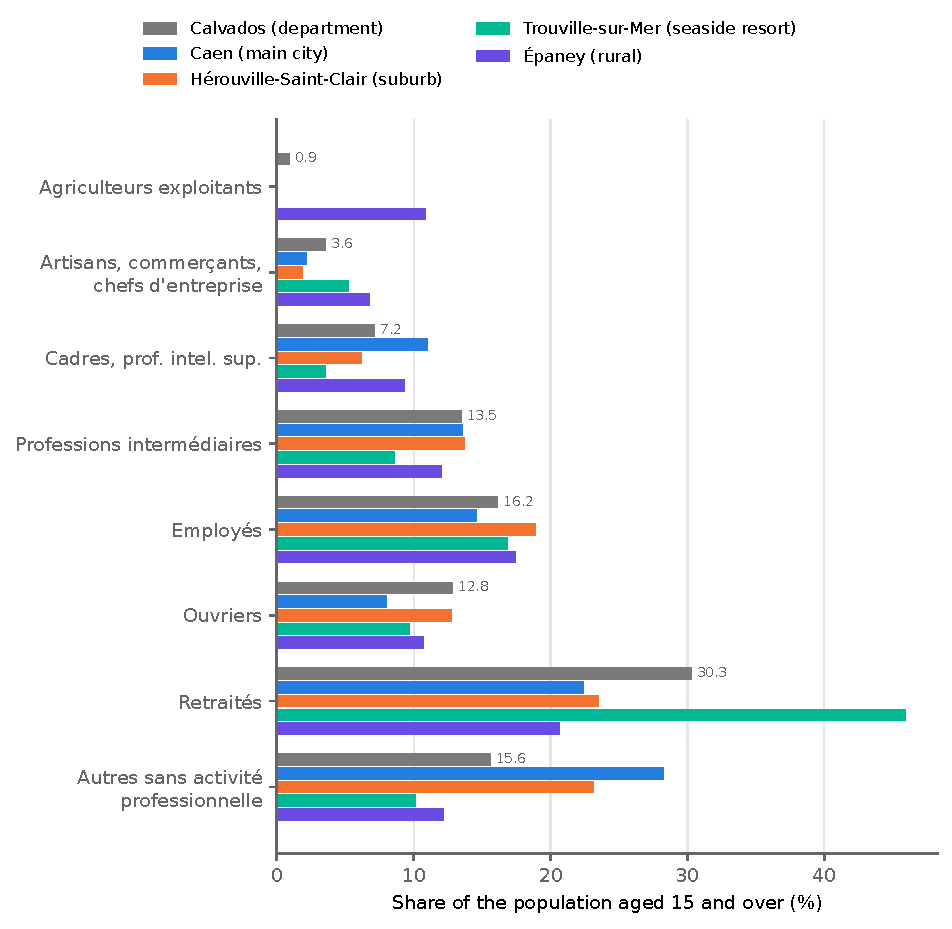
\includegraphics[width=0.9\textwidth]{spc_distribution}
  \caption{Socio-professional categories of the population aged 15 and over: Calvados (grey, reference, value
  labelled) and four municipalities. Shares in \%. Data: INSEE RP2019, aggregated census by
  IRIS~\cite{insee-census-aggregated} (department: identical shares in the weighted detailed
  census~\cite{insee-census-detailed}).}
  \label{fig:spc-distribution}
\end{figure}

\begin{table}[H]
  \centering
  \caption{Socio-professional categories of the population aged 15 and over (\%), Calvados and the four selected
  municipalities (aggregated census RP2019, \code{C19\_POP15P\_CS1} \dots\ \code{CS8}).}
  \label{tab:spc-shares}
  \small
  \begin{tabular}{@{}lrrrrr@{}}
    \toprule
    SPC & Calvados & Caen & H\'erouville & Trouville & \'Epaney \\
    \midrule
    1 Agriculteurs exploitants & 0.9 & 0.1 & 0.0 & 0.0 & 10.9 \\
    2 Artisans, commer\c{c}ants, chefs d'entreprise & 3.6 & 2.1 & 1.8 & 5.3 & 6.8 \\
    3 Cadres, professions intellectuelles sup. & 7.2 & 11.0 & 6.2 & 3.5 & 9.4 \\
    4 Professions interm\'ediaires & 13.5 & 13.5 & 13.7 & 8.6 & 12.0 \\
    5 Employ\'es & 16.2 & 14.6 & 18.9 & 16.9 & 17.4 \\
    6 Ouvriers & 12.8 & 8.0 & 12.7 & 9.7 & 10.7 \\
    7 Retrait\'es & 30.3 & 22.4 & 23.5 & 46.0 & 20.6 \\
    8 Autres sans activit\'e professionnelle & 15.6 & 28.2 & 23.1 & 10.1 & 12.2 \\
    \midrule
    Population 15+ & 576{,}234 & 92{,}552 & 18{,}560 & 4{,}076 & 370 \\
    \bottomrule
  \end{tabular}
\end{table}

\paragraph{Result.}
In the department as a whole, retirees are the largest group (30.3\,\%), followed by employ\'es (16.2\,\%), other
persons without professional activity (15.6\,\%), professions interm\'ediaires (13.5\,\%) and ouvriers (12.8\,\%);
farmers are 0.9\,\%. The municipalities differ clearly from this profile:
\begin{itemize}
  \item \textbf{Caen} has almost twice the department share of persons without professional activity (28.2 vs.\
  15.6\,\%), mostly students, more cadres (11.0 vs.\ 7.2\,\%), and fewer retirees (22.4 vs.\ 30.3\,\%) and ouvriers
  (8.0 vs.\ 12.8\,\%).
  \item \textbf{H\'erouville-Saint-Clair} shares the young profile of Caen (23.1\,\% without activity, 23.5\,\%
  retirees) but has more employ\'es (18.9\,\%) and fewer cadres (6.2\,\%) than both Caen and the department.
  \item \textbf{Trouville-sur-Mer} is dominated by retirees (46.0\,\%, 15.7 percentage points above the department);
  professions interm\'ediaires (8.6\,\%) and cadres (3.5\,\%) are well below the average, artisans and shopkeepers
  slightly above (5.3\,\%).
  \item \textbf{\'Epaney} has twelve times the department share of farmers (10.9 vs.\ 0.9\,\%), more artisans
  (6.8\,\%) and fewer retirees (20.6\,\%). Its shares rest on only 370 persons aged 15+ and are therefore less certain
  than those of the larger municipalities.
\end{itemize}
The SPC profiles match the age pattern of \cref{fig:mean-age-map}: the young urban municipalities have many students and
few retirees, the old coastal resort the reverse.

\paragraph{Problems encountered.}
\begin{itemize}
  \item \emph{Municipalities not identifiable in the detailed census.} Only 17 of 528 municipalities can be identified
  (\cref{sec:study-area}), so the map and the youngest and oldest municipality had to be computed from the aggregated
  census by IRIS. That file has only age bands, so the mean age per municipality is an estimate (band midpoints, 80+
  set to 85 years). We validated it on the 17 identifiable municipalities (\cref{tab:mean-age-validation}).
  \item \emph{Two age variables.} The detailed file has two single-year ages: \code{AGED}, the age reached during the
  census year, and \code{AGEREV}, the age in completed years. \code{AGED} is on average about one year higher. We use
  \code{AGEREV}: it is the usual meaning of age, and only with it do the weighted band totals of the detailed file match
  the age bands of the aggregated file (within 1.0\,\%, against up to 33\,\% with \code{AGED}). The shared census
  file of the project (\code{census\_14.parquet}, written in Exercise~1.1) therefore stores \code{AGEREV} as its
  age column; \code{AGED} is kept only for this comparison.
  \item \emph{Two exploitations of the census.} The population of the aggregated file (\code{P19\_POP},
  \emph{exploitation principale}) and the weights of the detailed file (\emph{exploitation compl\'ementaire}) differ
  slightly, by 0.03\,\% for the department and by up to about one year of mean age for single municipalities
  (Colombelles). The SPC counts of both files come from the same exploitation and agree exactly.
  \item \emph{SPC of children.} Persons under 15 carry \code{CS1 = 8}; all SPC shares therefore use the population 15+.
  A few observations aged 14 in completed years carry another SPC (they turn 15 in the census year). With
  \code{AGEREV} $\geq 15$ the detailed file reproduces the aggregated population 15+ exactly.
  \item \emph{Small municipalities.} Mean ages and SPC shares of very small municipalities rest on few persons. We
  therefore also report the youngest and oldest municipality among municipalities with at least 500 inhabitants and
  chose a rural example with at least 500 inhabitants.
\end{itemize}
